\subsubsection{Registracija kandidata}
\label{subsubsec:registracija}
\begin{itemize}
  \item \textbf{Kratak opis}: Da bi kandidat mogao da se uloguje na svoj nalog i vidi svoje podatke, nepohodno je da dobije potvrdu da je upisan u auto školu, kao i nepohodan ID za logovanje.
  \item \textbf{Učesnici}:
  \begin{itemize}
    \item Kandidat
    \item Administrator sistema
    \item Administrativni radnik.
  \end{itemize}
  \item \textbf{Preduslovi}:
    \begin{itemize}
    \item  Kandidat je popunio online prijavu.
    \item  Kandidat ispunjava uslove za upis.
    \end{itemize}
  \item \textbf{Postuslovi}:
      \begin{itemize}
      \item Kandidat je evidentiran u sistemu.
      \item Kandidat može da se prijavi na sistem.
      \end{itemize}
  \item \textbf{Osnovni tok}:
      \begin{enumerate}
        \item Administrator sistema prima informacije o novom kadnidatu.
        \item Administrator sistema unosi novog korisnika u bazu podataka.
        \item Sistem čuva unete podatke.
        \item Sistem šalje mejl novom kandidatu sa njegovim ID-jem.
        \item Sistem šalje mejl administrativnom radniku da je uspešno dodao novog kanidata.
        \item Administrativni radnik poziva kadnidata telefonom i proverava da li je dobio mejl sa svim potrebnim informacijama za prijavljivanje.
        \item Administrativni radnik ažurira spisak prijavljenih kandidata dodavanjem novog kadnidata.    
      \end{enumerate}

  \item \textbf{Alternativni tokovi}:
      \begin{itemize}
        \item A1. \textbf{Kandidat nije dobio mejl sa ID-jem i šifrom za pristupanje svom nalogu.}
        Ukoliko u koraku 4 kandidat nije dobio mejl, administrator sistema zahteva od sistema da ponovo pošalje mejl. Proces se nastavlja u koraku 4. osnovnog toka.
        \item A2. \textbf{Administrativni radnik ne može da kontaktira kadnidata.}
        Ukoliko u koraku 6 administrativni radnik ne može da stupi u kontakt sa kandidatom, trenutno stanje sistema se pamti i prekida se slučaj upotrebe na neko vreme. Naredni dan se slučaj upotrebe nastavlja ponovnim pozivom kandidata odnosno proces se nastavlja od 6. koraka osnovnog toka.
      \end{itemize}
\end{itemize}

\begin{figure}[H]
  \begin{center}
      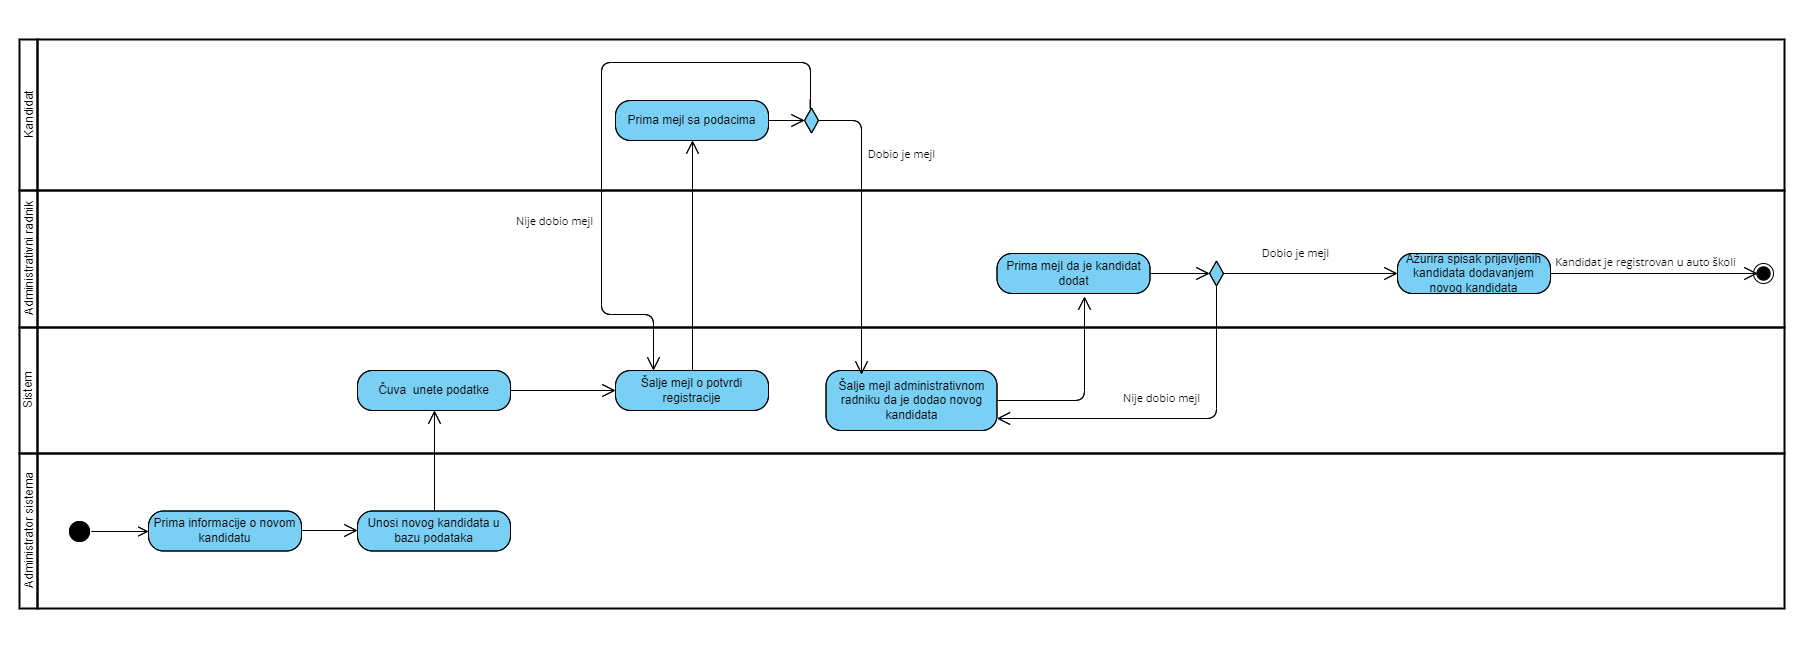
\includegraphics[width=140mm, height=70mm]{Diagrams/dijagram_aktivnosti_registracija_kandidata.png}
  \end{center}
  \caption {Dijagram aktivnosti - Registracija kandidata}
  \label{activity_registracija}

\end{figure}
